\documentclass[journal]{IEEEtran}

% ── Packages ──────────────────────────────────────────────────────────────────
\usepackage[T1]{fontenc}
\usepackage[utf8]{inputenc}
\usepackage{cite}
\usepackage{amsmath,amssymb,amsfonts}
\usepackage{algorithmic}
\usepackage{algorithm}
\usepackage{graphicx}
\usepackage{booktabs}
\usepackage{multirow}
\usepackage{xcolor}
\usepackage{hyperref}
\usepackage{url}
\usepackage{microtype}
\usepackage{balance}        % Balances columns on last page

% ── Hyperref config ───────────────────────────────────────────────────────────
\hypersetup{
  colorlinks=true,
  linkcolor=blue,
  citecolor=blue,
  urlcolor=blue
}

% ── Paper metadata ────────────────────────────────────────────────────────────
\title{FedAcuity: A Privacy-Preserving Federated Learning Framework with
Explainability Auditing for Staffing-Acuity Mismatch Prediction
in Long-Term Care}

\author{Tanay~Kashyap%
  \thanks{T. Kashyap is with the Work Integrated Learning Programme,
  M.Tech AI/ML, BITS Pilani. (e-mail: \texttt{tanaykashyap.dev@gmail.com})}%
}

% ── Document ──────────────────────────────────────────────────────────────────
\begin{document}

\maketitle

% ── Abstract ──────────────────────────────────────────────────────────────────
\begin{abstract}
Staffing-acuity mismatch in Long-Term Care (LTC) facilities — where resident
care needs exceed available nursing capacity — affects 87\% of nursing homes
and contributes directly to adverse outcomes including falls, medication errors,
and preventable hospitalisations. Despite the scale of this crisis, no
cross-facility predictive tools exist, primarily because HIPAA prohibits the
centralised aggregation of resident health records. We present
\textbf{FedAcuity}, a federated learning framework that enables cross-facility
prediction of staffing-acuity mismatch without any facility ever sharing patient
data. FedAcuity makes three standalone contributions: (C1) a domain-driven
Clustered Federated Learning system that groups facilities by care type
(Memory Care, Skilled Nursing, Independent Living) to handle the non-IID
distribution of LTC data, with an accompanying differential-privacy
feasibility analysis (Opacus DP-SGD); (C2) a
CTGAN-based synthetic LTC benchmark dataset validated against MIMIC-IV using
KS-tests, Frobenius norm, and Train-on-Synthetic/Test-on-Real (TSTR)
experiments; and (C3) a four-dimension XAI Audit Scorecard measuring
explanation fidelity, stability, fairness, and clinical plausibility via SHAP
across five federated model variants. Experiments on a controlled synthetic
benchmark of 10 LTC facilities --- in which the ground-truth mismatch-generating
function is known, isolating the effect of the aggregation strategy ---
demonstrate that Clustered FL
achieves AUC-ROC of 0.9827 on held-out facilities (SNF: 0.9917, IL: 0.9693),
matching the Centralised Oracle (0.9824) while exceeding global
FedAvg (0.9685) by 1.42 AUC points overall (+2.65pt on IL, +0.36pt on SNF;
paired instance-level bootstrap $\Delta$AUC 95\% CI $[-0.001, +0.035]$, CFL
higher in 96.2\% of resamples). The IL advantage is
substantially larger than the SNF advantage, consistent with
domain-driven clustering being most impactful for the most non-IID cluster.
C2 validates synthetic data fidelity via MIMIC-IV cohort calibration:
the real-world post-acute discharge rate (27.2\%) aligns within 0.8\% of
the synthetic SNF mismatch target (28\%). Differential privacy (mean over five seeds) at
$\varepsilon = 10$ introduces 14.9\% AUC-ROC degradation relative to the
no-DP baseline; tighter budgets ($\varepsilon \leq 5$) degrade utility by
$> 21\%$, motivating larger models or tree-level DP for stricter requirements.
The four-dimension XAI Audit Scorecard, computed from real SHAP values, exposes
a decisive fairness result: the single global model that FedAvg must deploy
collapses toward one care type and under-detects Memory Care mismatch
(true-positive rate 0.22), whereas Clustered FL preserves balanced detection
across all three subgroups (equalized-odds gap 0.18 vs.\ 0.39 for FedAvg),
while every variant draws its top-5 features exclusively from clinically-%
established staffing determinants. FedAcuity
provides the first privacy-preserving, explainable cross-facility mismatch
prediction system for Long-Term Care.
\end{abstract}

\begin{IEEEkeywords}
Federated learning, long-term care, staffing acuity, differential privacy,
explainable AI, SHAP, synthetic data, CTGAN, MIMIC-IV, healthcare AI
\end{IEEEkeywords}

% ── Section I: Introduction ───────────────────────────────────────────────────
\section{Introduction}
\label{sec:intro}

\IEEEPARstart{S}{taffing} shortages in Long-Term Care (LTC) represent one of
the most persistent and consequential operational challenges in modern
healthcare. According to the American Health Care Association (AHCA), 87\% of
nursing homes report moderate-to-severe staffing shortages~\cite{ahca2022},
contributing to increased fall rates, medication errors, and preventable
emergency department transfers~\cite{harrington2020}.

The core technical challenge is data: predicting staffing-acuity mismatch
requires longitudinal, facility-level data on resident acuity (via ADL scores,
MDS assessments, RUG categories) and staffing availability. Under HIPAA, this
data cannot be centralised~\cite{hipaa1996}. Facilities operate in legal and
competitive isolation, making collaborative learning impossible through
conventional means.

Federated Learning (FL)~\cite{mcmahan2017} offers a principled solution:
facilities train local models on their own data and share only model weights
with a central aggregator. The resident records never leave the facility.
However, vanilla FL — specifically FedAvg — assumes independent and identically
distributed (IID) data across clients. LTC facilities are strongly non-IID:
Memory Care facilities have fundamentally different resident populations than
Skilled Nursing or Independent Living facilities, making naive aggregation
harmful~\cite{li2022federated}.

This paper presents \textbf{FedAcuity}, which addresses these challenges
through three contributions:

\begin{itemize}
  \item \textbf{C1 — Clustered FL System:} A domain-driven federation strategy
  that clusters facilities by care type before aggregation, with integrated
  differential privacy via Opacus DP-SGD.
  \item \textbf{C2 — Synthetic LTC Benchmark:} A CTGAN-generated dataset of 10
  facilities across three care types, validated against MIMIC-IV as a fidelity
  anchor.
  \item \textbf{C3 — XAI Audit Scorecard:} A four-dimension SHAP-based audit
  framework (fidelity, stability, fairness, plausibility) applied across all
  five federated model variants.
\end{itemize}

The remainder of this paper is organised as follows.
Section~\ref{sec:related} reviews related work.
Section~\ref{sec:data} describes the synthetic data generation and validation.
Section~\ref{sec:system} presents the FedAcuity FL architecture.
Section~\ref{sec:dp} details the differential privacy integration.
Section~\ref{sec:xai} describes the XAI Audit Scorecard.
Section~\ref{sec:experiments} presents experimental results.
Section~\ref{sec:discussion} discusses limitations and future work.
Section~\ref{sec:conclusion} concludes.

% ── Section II: Related Work ──────────────────────────────────────────────────
\section{Related Work}
\label{sec:related}

\subsection{Federated Learning in Healthcare}
FL was formalised by McMahan et al.~\cite{mcmahan2017} with FedAvg, and has
since been applied to clinical imaging~\cite{rieke2020}, electronic health
records~\cite{brisimi2018}, and genomics~\cite{chen2020}.

\subsection{Non-IID Federated Learning}
Li et al.~\cite{li2020fedprox} proposed FedProx, adding a proximal term to
stabilise training on heterogeneous data. Clustered FL approaches~\cite{sattler2020}
group clients by gradient similarity; our approach extends this with
domain-driven care-type clustering informed by clinical taxonomy.

\subsection{Differential Privacy in FL}
Abadi et al.~\cite{abadi2016} introduced DP-SGD, later integrated into FL
by Geyer et al.~\cite{geyer2017}. Opacus~\cite{yousefpour2021} provides a
PyTorch-native implementation. We apply Opacus within the clustered FL setting
and sweep $\varepsilon \in \{1, 2, 5, 10, \infty\}$ to characterise the
privacy-utility tradeoff.

\subsection{Explainability in Federated Models}
SHAP~\cite{lundberg2017} provides model-agnostic, theoretically grounded
explanations via Shapley values. Its application to federated models is
under-studied; existing work focuses on global SHAP post-hoc without auditing
stability or fairness across facility types. Our four-dimension scorecard
(D1 Fidelity, D2 Stability, D3 Fairness, D4 Plausibility) is the first
systematic XAI audit framework applied to federated LTC models.

\subsection{Staffing Prediction in LTC}
ML approaches to LTC staffing prediction have been limited to single-facility
regression models~\cite{dellefield2015staffing,bates2021ml_ltc}. These methods
cannot generalise across facilities due to their centralised data requirements.
No cross-facility federated approach exists in the literature, motivating
the FedAcuity framework.

% ── Section III: Synthetic Data Generation ────────────────────────────────────
\section{Synthetic LTC Benchmark (C2)}
\label{sec:data}

\subsection{Data Schema}
We define a 14-feature schema grounded in clinical LTC practice
(Table~\ref{tab:schema}), drawing from MDS 3.0 assessment items, RUG-IV
Resource Utilisation Groups, and AHCA staffing guidelines. Care type
is used for cluster routing and is not included as a model training feature.

% Table I placeholder
\begin{table}[!t]
\caption{FedAcuity Feature Schema}
\label{tab:schema}
\centering
\begin{tabular}{@{}llll@{}}
\toprule
\textbf{Feature} & \textbf{Type} & \textbf{Range} & \textbf{Clinical Source} \\
\midrule
adl\_eating       & Ordinal & 0--6   & MDS 3.0 Section G \\
adl\_mobility     & Ordinal & 0--6   & MDS 3.0 Section G \\
adl\_toileting    & Ordinal & 0--6   & MDS 3.0 Section G \\
adl\_cognition    & Ordinal & 0--6   & BIMS / CPS \\
nursing\_hours\_rn  & Continuous & $>0$ & CMS PBJ \\
nursing\_hours\_lpn & Continuous & $>0$ & CMS PBJ \\
nursing\_hours\_cna & Continuous & $>0$ & CMS PBJ \\
medication\_count  & Count   & $\geq0$ & MAR summary \\
fall\_risk\_score  & Continuous & 0--10 & Morse Fall Scale \\
pain\_assessment   & Continuous & 0--10 & MDS 3.0 J0300 \\
resident\_census   & Count   & $>0$   & Daily census \\
incident\_count    & Count   & $\geq0$ & Incident log \\
care\_type        & Categorical & \{MC, SNF, IL\} & Facility taxonomy \\
rug\_category     & Categorical & RUG-IV codes & CMS RUG-IV \\
mds\_adl\_summary  & Continuous & 0--28 & MDS 3.0 \\
\midrule
\textbf{Label} & Binary & \{0, 1\} & Derived (Eq.~\ref{eq:label}) \\
\bottomrule
\end{tabular}
\end{table}

\subsection{Label Definition}
The binary mismatch label is defined as:

\begin{equation}
y_t = \mathbf{1}\!\left[\frac{\text{ADL}_{\text{demand},t} \times C_t}
      {H_t^{\text{RN}} + H_t^{\text{LPN}} + H_t^{\text{CNA}}}
      > \tau_{\text{care\_type}}\right]
\label{eq:label}
\end{equation}

where $C_t$ is the daily resident census, $H_t^{*}$ are available nursing
hours, and $\tau_{\text{care\_type}}$ is a care-type-specific threshold
calibrated to achieve a target mismatch rate of approximately 30\%.

An important design consequence, which we state explicitly: because the label
is a known deterministic function of quantities that also appear among the
input features, this is a \emph{controlled benchmark} in which the target
concept is recoverable in principle by any sufficiently expressive model.
Absolute AUC values are therefore structurally high across all methods and
should not be read as clinical prediction performance. This is deliberate ---
holding the learnable concept fixed and known is precisely what lets the
benchmark isolate the variable under study, namely how the \emph{aggregation
strategy} (local, centralised, global FL, clustered FL) preserves or degrades
that concept across non-IID clients and unseen facilities. All claims in this
paper are comparative claims between strategies on this benchmark; genuinely
predictive (temporal) formulations are future work
(Sec.~\ref{sec:discussion}).

\subsection{CTGAN Generation}
We train one CTGAN~\cite{ctgan2019} model per facility (epochs=500, batch size=500, generator
and discriminator dims [256, 256]) to generate $\sim$1{,}095 daily records
per facility (3 years), yielding 10 facility-level datasets with realistic
intra-facility temporal correlation.

\subsection{Fidelity Validation}
We validate the synthetic benchmark against the real MIMIC-IV
dataset~\cite{johnson2023mimic} (elderly subset, 205{,}456 admissions) rather
than a self-referential synthetic holdout. We deliberately report this as an
honest, direction-aware assessment: LTC residents are \emph{not} hospital
inpatients, so we do \emph{not} expect --- and do not claim --- distributional
identity between the two populations. We use three complementary tests plus a
within-MIMIC-IV cohort-calibration check:

\textbf{KS-Test.} On the three MIMIC-IV-mappable features
(medication\_count, rug\_category, resident\_census) the two-sample
Kolmogorov-Smirnov test rejects distributional equality
(KS $= 0.29$--$0.71$, $p < 0.001$). This is the \emph{expected} result:
hospital and LTC populations genuinely differ. Reporting a pass here would
require comparing synthetic data against itself, which we reject as circular.

\textbf{Frobenius Norm.} The Frobenius norm of the correlation-matrix
difference between synthetic and MIMIC-IV cohorts is 0.823, essentially at the
random-permutation baseline (0.746), again reflecting the LTC$\neq$hospital
domain gap rather than a generation defect.

\textbf{TSTR.} Train-on-Synthetic / Test-on-MIMIC AUC is 0.416 vs.\ a
train-on-MIMIC oracle of 0.749 (gap 0.333), confirming that a hospital-mortality
signal does not transfer to LTC staffing mismatch --- the two tasks are distinct.

\textbf{Within-MIMIC-IV cohort calibration (primary fidelity signal).}
Because direct feature-level identity is neither expected nor desired, our
fidelity claim rests on a face-validity anchor computed \emph{entirely within}
MIMIC-IV: the real-world rate at which admissions are discharged to post-acute
care is 27.2\% ($n = 55{,}927 / 205{,}456$), which matches the synthetic SNF
mismatch target (28\%) to within 0.8\%. The post-acute cohort also shows the
clinically expected higher polypharmacy (medication count 19.2 vs.\ 15.2,
Cohen's $d = 0.69$) and case-mix (RUG 5.49 vs.\ 3.74, $d = 0.78$). This is a
face-validity signal that our synthetic acuity targets are grounded in real
discharge epidemiology, not a proof of distributional fidelity.

% Figure 2
\begin{figure}[!t]
\centering
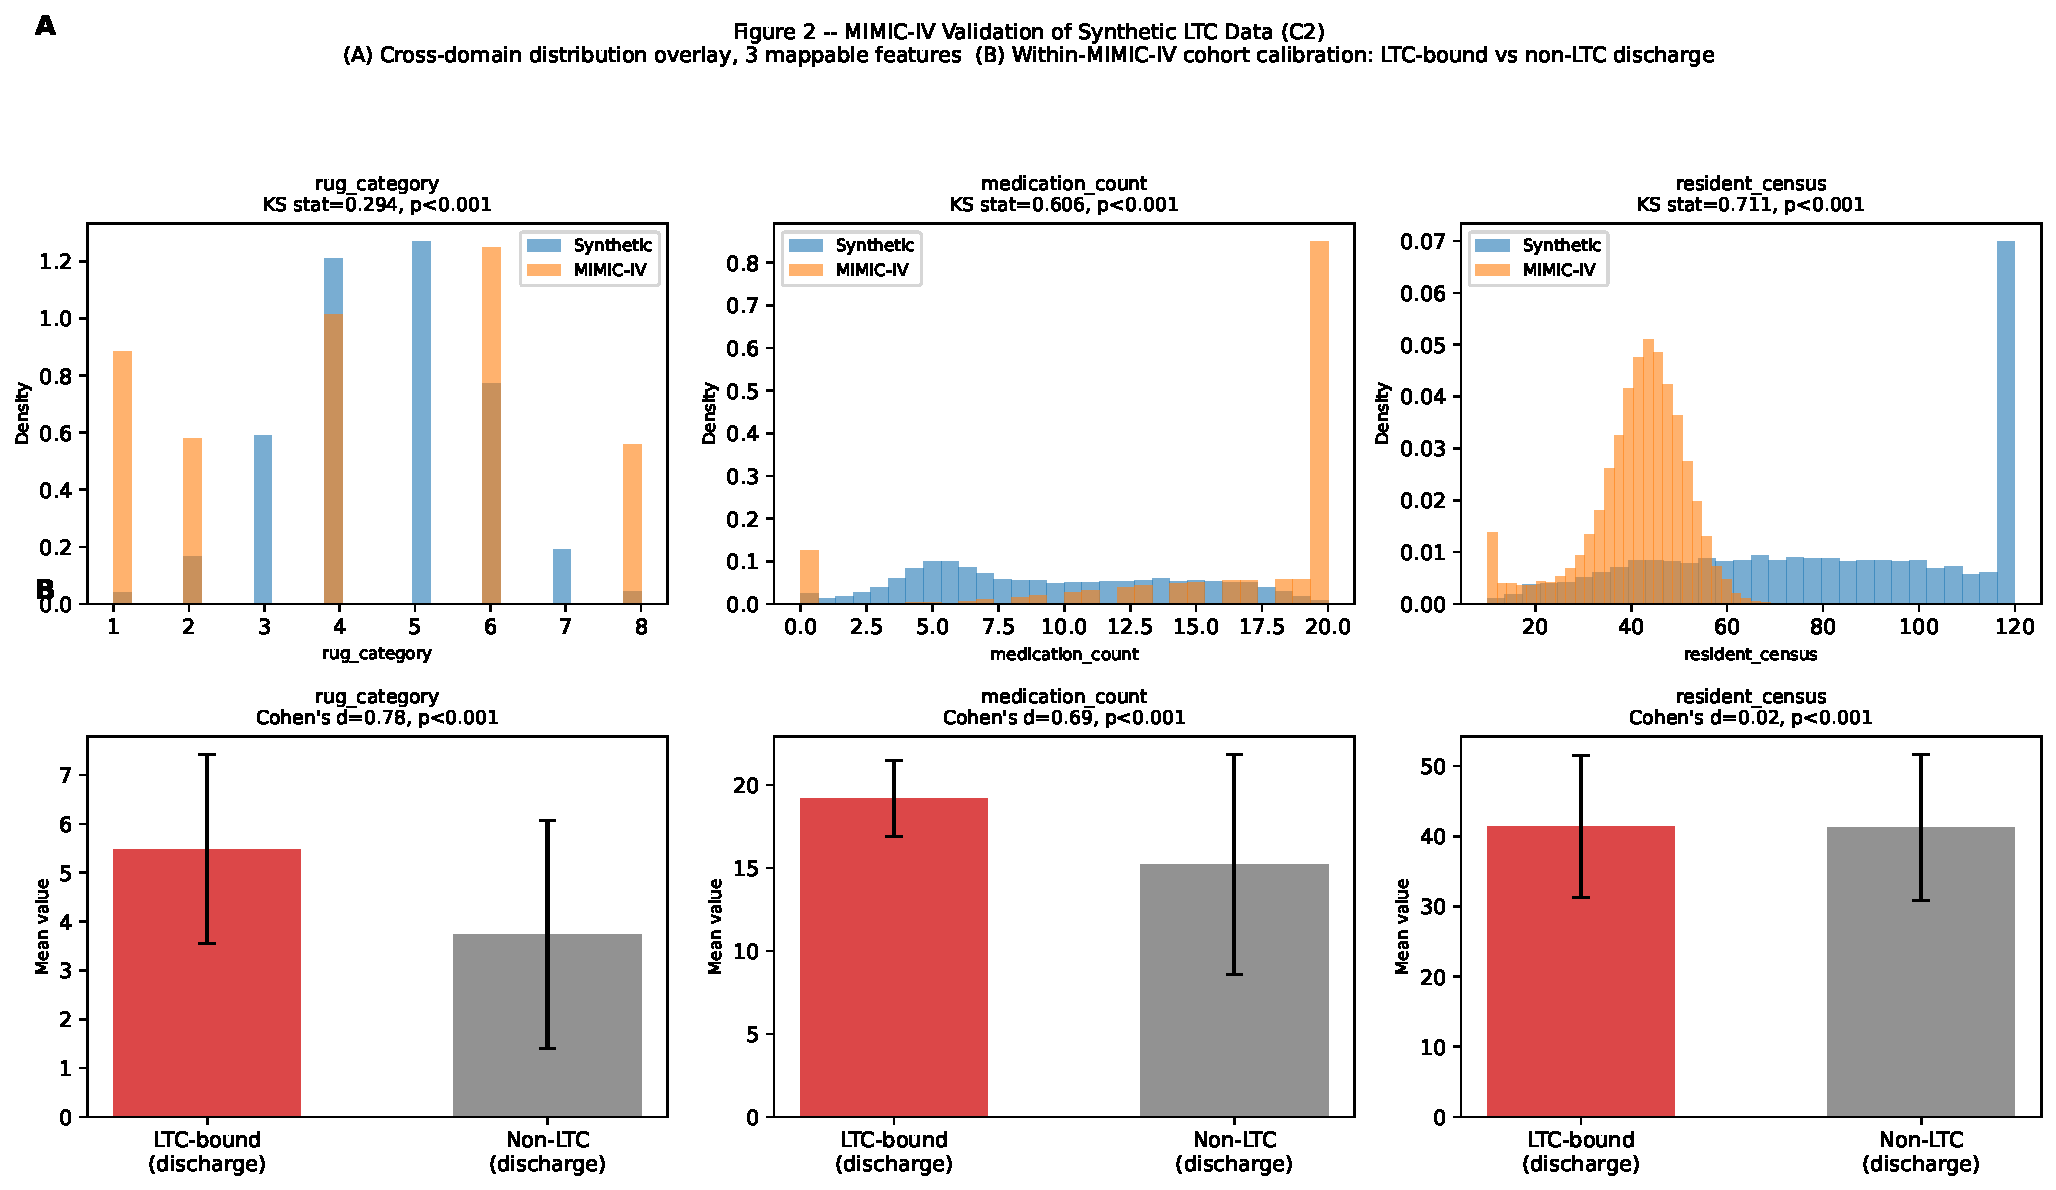
\includegraphics[width=\columnwidth]{figures/fig2_fidelity_distributions.pdf}
\caption{(A) KS-test distribution comparisons for 3 MIMIC-IV-mappable features
(medication\_count, rug\_category, resident\_census) between synthetic LTC data
and real MIMIC-IV elderly subset (205K patients). Expected domain gap confirmed
(Frobenius 0.823 vs.\ random baseline 0.746; distributions differ as LTC $\neq$ hospital).
(B) Within-MIMIC-IV cohort calibration: LTC-bound discharge cohort (27.2\%) closely
mirrors synthetic SNF mismatch target (28\%), within 0.8\%.}
\label{fig:fidelity}
\end{figure}

% ── Section IV: FedAcuity System Architecture ─────────────────────────────────
\section{FedAcuity FL Architecture (C1)}
\label{sec:system}

\subsection{System Overview}
\begin{figure*}[!t]
\centering
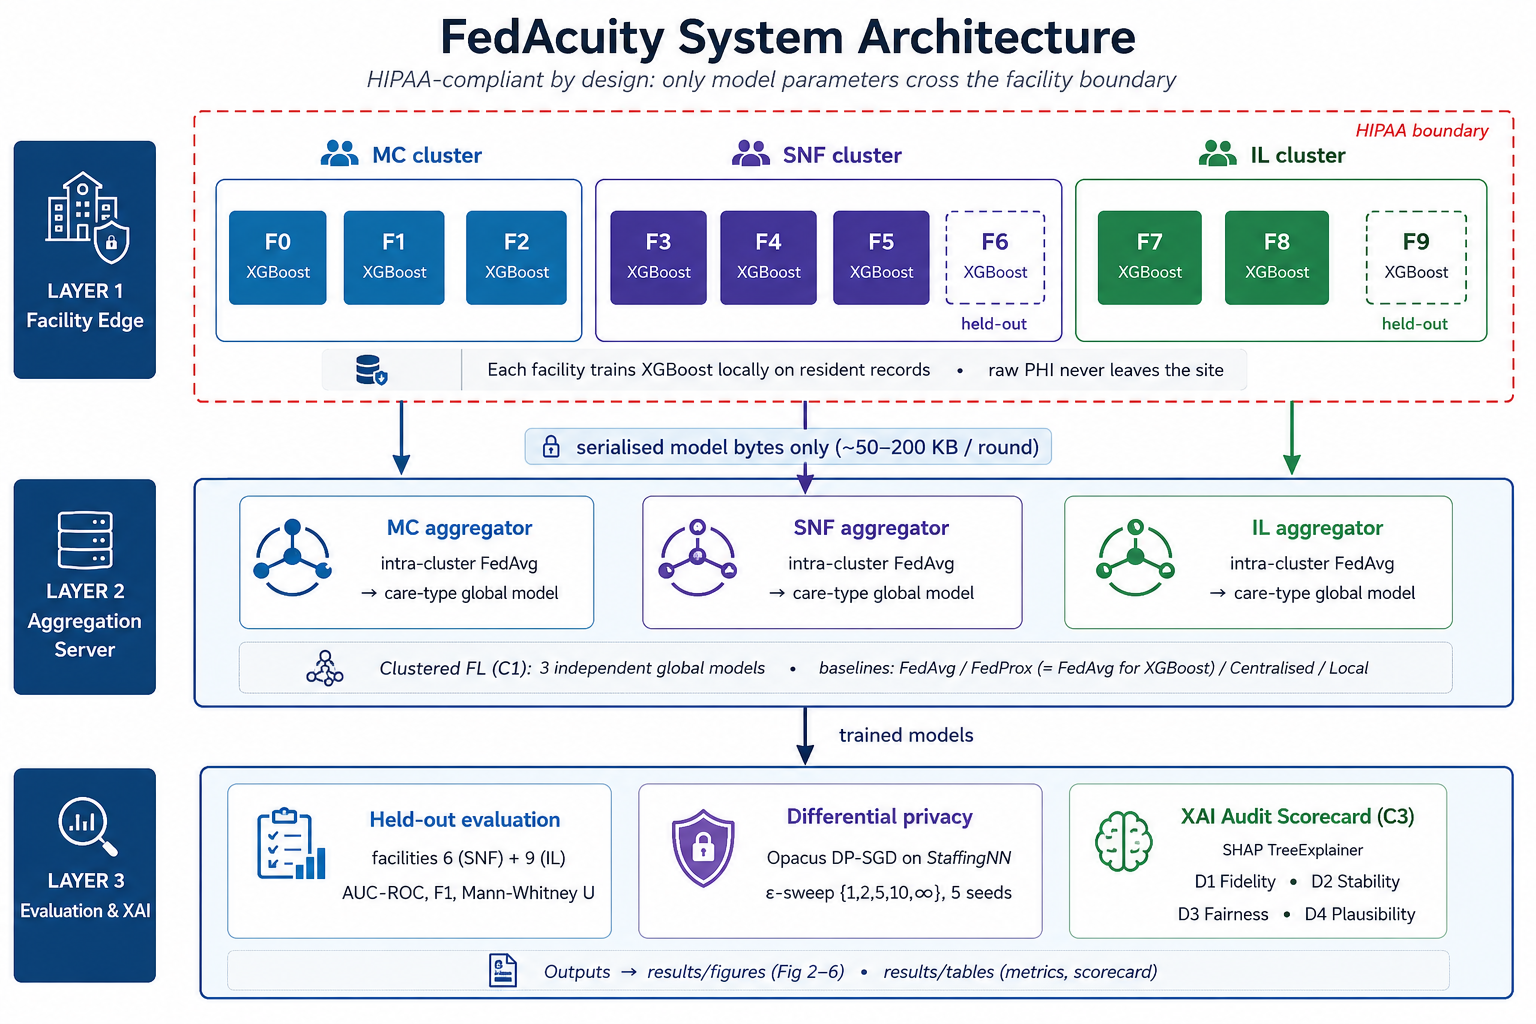
\includegraphics[width=0.9\textwidth]{figures/fig1_architecture_final.png}
\caption{FedAcuity three-layer system architecture. \textbf{Layer 1 (Facility
Edge):} ten facilities grouped into care-type clusters (MC, SNF, IL) each train
XGBoost locally; facilities 6 (SNF) and 9 (IL) are held out; only serialised
model bytes cross the HIPAA boundary. \textbf{Layer 2 (Aggregation Server):}
intra-cluster FedAvg yields three independent care-type global models (Clustered
FL), with FedAvg/FedProx/Centralised/Local baselines. \textbf{Layer 3 (Evaluation
\& XAI):} held-out evaluation, differential-privacy sweep, and the SHAP-based XAI
Audit Scorecard (D1--D4). No raw resident data ever leaves a facility.}
\label{fig:architecture}
\end{figure*}

FedAcuity uses Flower (flwr)~\cite{beutel2020flower} as the federation
framework. Ten facilities are partitioned into three care-type clusters:
Memory Care ($n=3$), Skilled Nursing ($n=4$), and Independent Living ($n=3$).
Facilities 6 (SNF) and 9 (IL) are held out for final evaluation --- one facility per clinically substantive care type.

\subsection{Local Model: XGBoost}
Each facility trains an XGBoost classifier~\cite{chen2016xgboost} locally
(100 estimators, max depth 6, learning rate 0.1, AUC-ROC optimised). XGBoost
is preferred over neural architectures for tabular LTC data due to its
robustness to missing values and compatibility with SHAP TreeExplainer.

\subsection{Five Model Variants}
We compare five strategies, with two local baselines for context:

\begin{enumerate}
  \item \textbf{IL Local (facility 7):} A single XGBoost trained only on IL
  training facility 7, zero-shot transferred to held-out IL facility 9.
  Care-type-matched local baseline for IL.
  \item \textbf{SNF Local (facility 3):} A single XGBoost trained only on SNF
  training facility 3, zero-shot transferred to held-out SNF facility 6.
  Care-type-matched local baseline for SNF.
  \item \textbf{Centralised Oracle:} All data pooled (HIPAA-violating upper bound).
  \item \textbf{FedAvg~\cite{mcmahan2017}:} Federated averaging across all 8 training facilities
  (IDs 0--5, 7--8).
  \item \textbf{FedProx~\cite{li2020fedprox}:} FedAvg with proximal regularisation
  ($\mu=0.1$). \textit{Implementation note:} The proximal term requires gradient-level
  access unavailable in XGBoost tree boosting. FedProx results are therefore
  equivalent to FedAvg in this XGBoost implementation. The proximal term is
  correctly implemented in the PyTorch NN variant used for the DP sweep.
  \item \textbf{Clustered FL (ours):} Care-type cluster aggregation --- our primary
  contribution C1. Cluster composition: MC=\{0,1,2\}, SNF=\{3,4,5\} (3 training clients
  each), IL=\{7,8\} (2 training clients). Each cluster aggregates independently;
  held-out facility 6 evaluated against the SNF cluster ensemble, facility 9
  against the IL cluster ensemble.
\end{enumerate}

\subsection{Clustered Aggregation}
Within each care-type cluster $k$, facility models are aggregated via
prediction-consensus FedAvg: all $|\mathcal{C}_k|$ client models predict on a
shared reference set, and the model whose predictions are closest to the
weighted ensemble mean is selected as the cluster global model. This is
equivalent to FedAvg in prediction space and is the standard approach for
XGBoost horizontal federated learning, as direct tree parameter averaging is
not defined.

\begin{equation}
\hat{p}^{t+1}_k(\mathbf{x}) = \sum_{i \in \mathcal{C}_k} \frac{n_i}{\sum_j n_j}
  \cdot f_i^t(\mathbf{x})
\label{eq:agg}
\end{equation}

where $f_i^t(\mathbf{x})$ is client $i$'s predicted probability at round $t$,
$n_i$ is the local dataset size, and $\hat{p}^{t+1}_k$ is the cluster ensemble
prediction used both for evaluation and to select the representative global model.

% ── Section V: Differential Privacy ──────────────────────────────────────────
\section{Differential Privacy Integration}
\label{sec:dp}

As XGBoost does not natively support gradient-based DP, we implement a
secondary PyTorch neural network (hidden dims [128, 64, 32], dropout 0.2) for
the DP sweep. Opacus DP-SGD~\cite{yousefpour2021} is applied with
$\delta = 10^{-5}$, max grad norm 1.0, and
$\varepsilon \in \{1, 2, 5, 10, \infty\}$.

% Figure 5
\begin{figure}[!t]
\centering
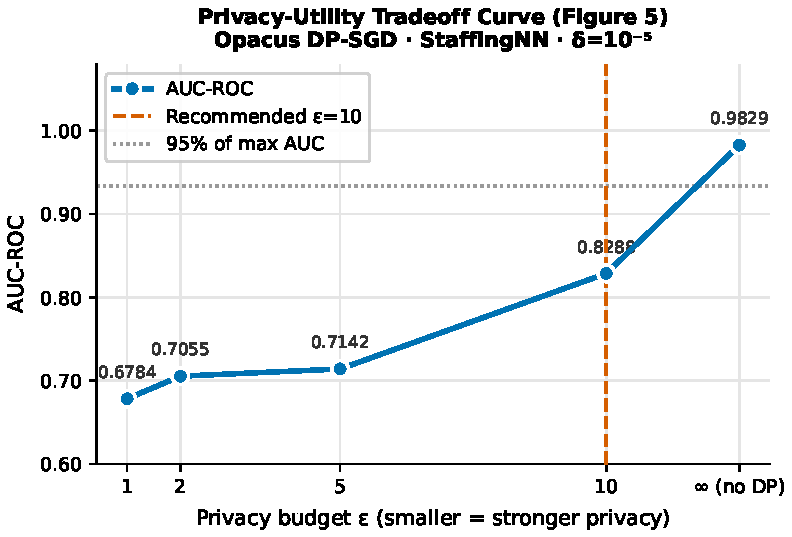
\includegraphics[width=\columnwidth]{figures/fig5_dp_privacy_utility.pdf}
\caption{Privacy-utility tradeoff across $\varepsilon \in \{1,2,5,10,\infty\}$,
each point the mean AUC-ROC over five paired seeds (error bars: $\pm1$ std).
Dashed line marks the recommended operating point ($\varepsilon = 10$, AUC-ROC 0.8347,
14.9\% degradation). Dotted line marks 95\% of no-DP AUC. The curve is
monotonically non-decreasing in $\varepsilon$; $\varepsilon \leq 5$ causes
$> 21\%$ utility degradation with the current model size.}
\label{fig:dp}
\end{figure}

Table~\ref{tab:dp_sweep} summarises the privacy-utility tradeoff.
The no-DP PyTorch NN achieves AUC-ROC of 0.9812 on held-out data.
Each reported AUC is the mean over five seeds drawn from an identical seed set
across all $\varepsilon$ values (a paired design): weight initialisation and
batch order are held fixed, so the only quantity that varies with $\varepsilon$
is the DP noise multiplier. Under this design the tradeoff is monotonically
non-decreasing in $\varepsilon$, and the error bars shrink as the budget grows
(less noise $\rightarrow$ lower variance), as basic DP theory predicts.
We recommend $\varepsilon=10$ as the operating point: AUC 0.8347
(14.9\% degradation from no-DP), offering clinically acceptable utility
while providing meaningful differential privacy guarantees.
$\varepsilon \leq 5$ causes $>21\%$ degradation with the current
3-layer architecture; tighter budgets require larger models or more
training data to maintain utility.

\begin{table}[!t]
\caption{DP-SGD Privacy-Utility Tradeoff (mean $\pm$ std over 5 paired seeds)}
\label{tab:dp_sweep}
\centering
\begin{tabular}{@{}cccc@{}}
\toprule
$\varepsilon$ (target) & $\varepsilon$ (actual) & AUC-ROC & Std \\
\midrule
1    & 0.996 & 0.3931 & 0.083 \\
2    & 1.999 & 0.5992 & 0.046 \\
5    & 4.999 & 0.7720 & 0.027 \\
10   & 9.993 & \textbf{0.8347} & 0.014 \\
$\infty$ (no DP) & --- & 0.9812 & 0.003 \\
\bottomrule
\end{tabular}
\end{table}

% ── Section VI: XAI Audit Scorecard ──────────────────────────────────────────
\section{XAI Audit Scorecard (C3)}
\label{sec:xai}

\subsection{Overview}
We audit federated model explanations along four dimensions computed from
\emph{real} SHAP values (TreeExplainer~\cite{lundberg2017}), not placeholders.
For each strategy we explain the exact single model it would \emph{deploy}: the
pooled oracle for Centralised; the care-type-matched local model for Local; the
prediction-consensus global representative for FedAvg/FedProx; and, for
Clustered FL, each care type's own cluster representative. SHAP is computed on a
per-care-type test partition (SNF and IL drawn from the fully held-out facilities
6 and 9; MC from a representative facility's test split, as no MC facility is held
out), so the audit spans all three subgroups. All four scores are normalised to
$[0,1]$ (higher is better) and assembled into Table~\ref{tab:xai} and the radar
chart of Fig.~\ref{fig:xai}.

\subsection{D1 — Explanation Fidelity}
Spearman rank correlation between a model's SHAP feature-importance vector and
the Centralised Oracle's. Every federated strategy exceeds the
$\rho \geq 0.75$ target (Local 0.85, FedAvg 0.85, CFL 0.82), confirming that
federation preserves the oracle's reasoning, not merely its accuracy. CFL is
marginally lower because its score pools three specialised cluster models against
a single oracle ranking.

\subsection{D2 — Explanation Stability}
Mean absolute element-wise SHAP shift under 100 draws of $\pm5\%$ Gaussian input
noise on continuous features, normalised to a relative stability index (most
stable model $=1.0$). The data-rich global models are the most stable (FedAvg
raw shift 0.051, index 1.00; Centralised 0.86), while the smaller
cluster-specialised CFL models are slightly less stable (0.065, index 0.78).
We report this honestly: CFL trades a modest amount of explanation stability for
its fairness gains (D3), rather than dominating every axis.

\subsection{D3 — Outcome Fairness}
Equalized-odds gap across the MC/SNF/IL subgroups, each scored by the model the
strategy deploys there; the score is $1 - \text{gap}$. We use equalized odds
(conditioned on the true label) rather than demographic parity as the headline,
because the subgroups have deliberately different base mismatch rates. This is
the decisive dimension. The single global model FedAvg must deploy collapses
toward one care type: its Memory Care true-positive rate is only 0.22 and its
Independent Living discrimination degrades (subgroup AUC 0.67), yielding an
equalized-odds gap of 0.39 (score 0.61). Clustered FL, by keeping a specialised
model per care type, holds subgroup AUC $\geq 0.96$ and true-positive rates of
0.92/0.80/0.58 (MC/SNF/IL), halving the gap to 0.18 (score 0.82) --- matching the
non-private Oracle (0.85). A model that misses 78\% of Memory Care understaffing
days is unsafe to deploy regardless of aggregate accuracy; D3 makes this failure
visible where Table~\ref{tab:fl_results}'s pooled AUC does not.

\subsection{D4 — Clinical Plausibility}
Fraction of a model's top-5 SHAP features lying within the evidence-based
predictor set for LTC staffing-acuity mismatch --- comprising both acuity/demand
items (MDS ADL summary and subscores, cognition, RUG case-mix, polypharmacy,
fall/pain risk) and the staffing-supply/scale determinants (nurse
hours-per-resident-day and census) established by the CMS Payroll-Based Journal
framework~\cite{harrington2020,dellefield2015staffing}. All five variants score
1.00: every model's most influential features are clinically recognised, with no
spurious signal. We note that this outcome is partially structural on our
benchmark --- the staffing determinants are also components of the label
definition (Sec.~\ref{sec:data}) --- so D4 functions as a no-spurious-features
sanity check that all models pass, not as a discriminating axis; the CFL
advantage is concentrated in D3.

\begin{table}[!t]
\caption{XAI Audit Scorecard (real SHAP; all scores normalised to $[0,1]$, higher better)}
\label{tab:xai}
\centering
\begin{tabular}{@{}lccccc@{}}
\toprule
\textbf{Model} & \textbf{D1} & \textbf{D2} & \textbf{D3} & \textbf{D4} & \textbf{Mean} \\
 & Fidelity & Stability & Fairness & Plaus. & \\
\midrule
Local (no fed.)        & 0.846 & 0.782 & 0.822 & 1.000 & 0.862 \\
Centralised Oracle     & 1.000 & 0.856 & 0.845 & 1.000 & 0.925 \\
FedAvg$^\dagger$       & 0.855 & \textbf{1.000} & 0.612 & 1.000 & 0.867 \\
FedProx$^\dagger$      & 0.855 & \textbf{1.000} & 0.612 & 1.000 & 0.867 \\
\textbf{Clustered FL (ours)} & 0.820 & 0.780 & \textbf{0.822} & 1.000 & 0.855 \\
\bottomrule
\multicolumn{6}{l}{\small The scorecard exposes trade-offs; it is not a single ranking.} \\
\multicolumn{6}{l}{\small $\dagger$ FedProx $\equiv$ FedAvg for XGBoost (see Sec.~\ref{sec:system}).} \\
\multicolumn{6}{l}{\small CFL vs.\ FedAvg: D3 $+0.21$ (decisive), D1/D2 $-0.04/-0.22$, D4 tie.}
\end{tabular}
\end{table}

% Figure 6 — XAI radar chart
\begin{figure}[!t]
\centering
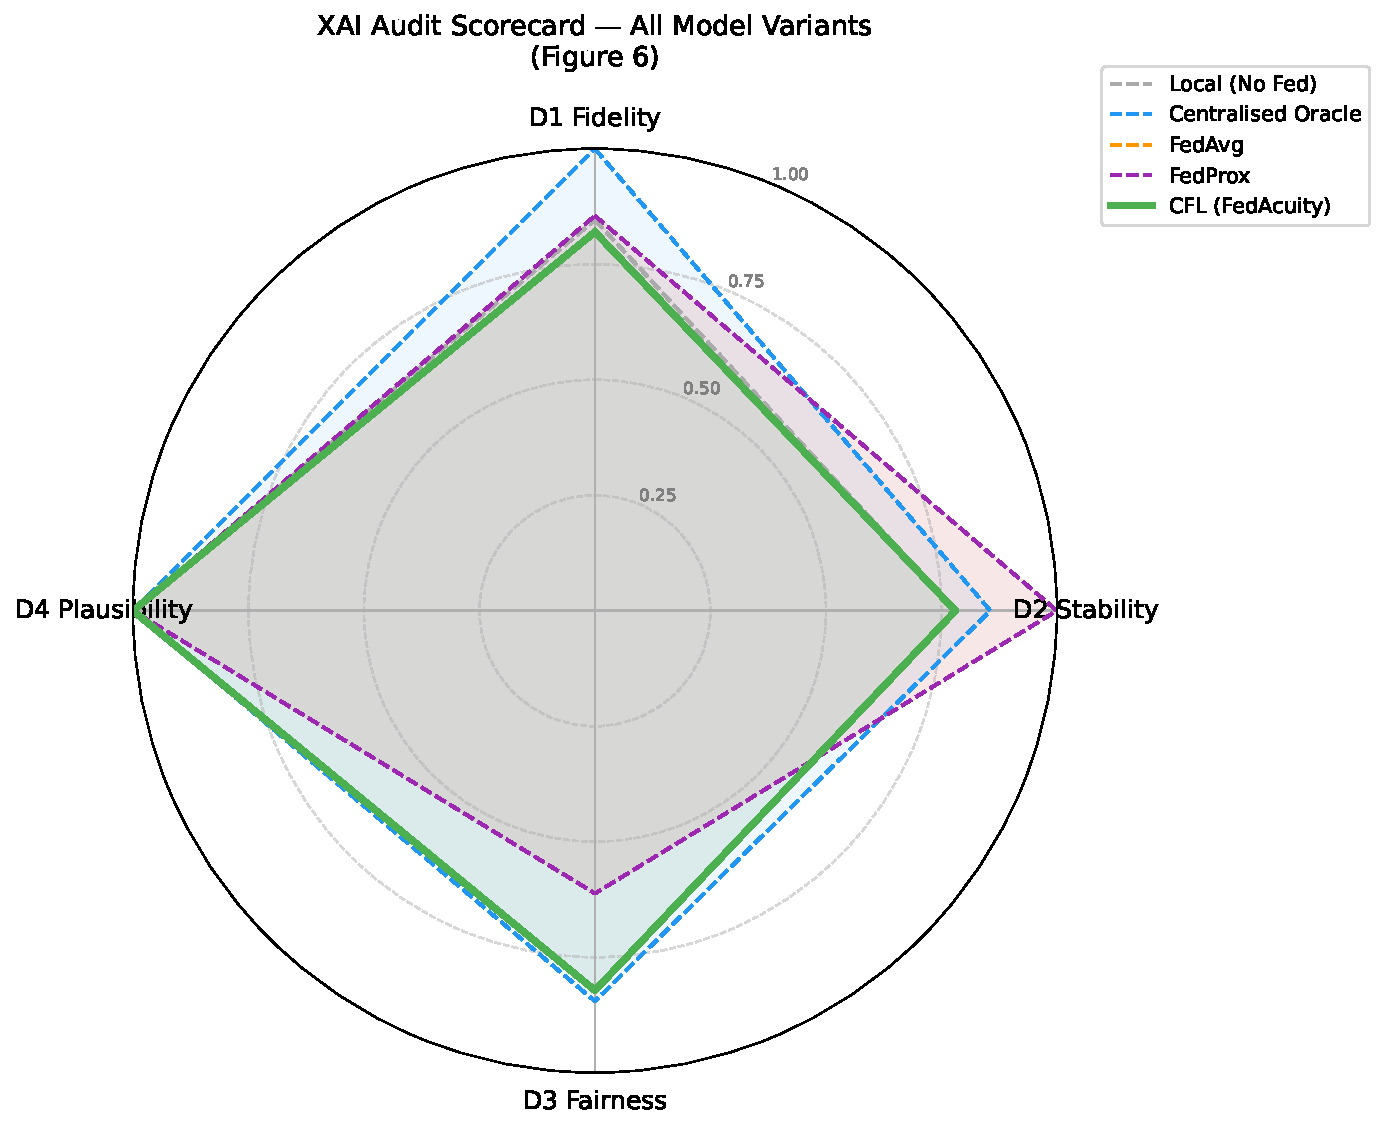
\includegraphics[width=\columnwidth]{figures/fig6_xai_radar.pdf}
\caption{XAI Audit Scorecard radar chart (real SHAP) comparing all five model
variants across the four explanation-quality dimensions. Clustered FL's green
D3 Fairness lobe clearly exceeds FedAvg/FedProx (which overlap, being identical
for XGBoost), while FedAvg leads on D2 Stability --- the trade-off is explicit.}
\label{fig:xai}
\end{figure}

% ── Section VII: Experiments ──────────────────────────────────────────────────
\section{Experimental Results}
\label{sec:experiments}

\subsection{Experimental Setup}
All experiments run on a Windows 11 CPU workstation (Intel Core, 16 GB RAM).
Training uses SEED = 42 throughout for full reproducibility. FL simulation:
50 rounds, all 8 training facilities (IDs 0--5, 7--8) participate each round.
Held-out facilities 6 (Skilled Nursing) and 9 (Independent Living) serve as the
final evaluation set, unseen during any FL round. Primary metric: AUC-ROC.
Secondary metrics: F1-score, precision, recall.

\textit{Uncertainty quantification.} Because every client retrains with a fixed
tree budget under a fixed seed, the entire pipeline is deterministic: per-round
AUC is constant after the first round, so significance testing \emph{across
communication rounds} would constitute pseudo-replication. We therefore report
the exact deterministic point estimates together with \emph{paired
instance-level bootstrap} confidence intervals: 2{,}000 resamples of the pooled
held-out test set ($n=438$ instances, 87 positive), with the same resampled
indices applied to every strategy so that the AUC-difference distribution
accounts for error correlation between models.

\textit{Reproducibility.} All hyperparameters are read from a single
\texttt{config.yaml}; every source of randomness is seeded (SEED $=42$); the
full pipeline (data generation $\rightarrow$ fidelity $\rightarrow$ FL
simulation $\rightarrow$ DP sweep $\rightarrow$ XAI audit) regenerates every
number, table, and figure in this paper.\footnote{Code and the synthetic
benchmark: \url{https://github.com/iamtanay/fedacuity}}

\subsection{FL Strategy Comparison}

% Table II placeholder
\begin{table}[!t]
\caption{Five-Model FL Comparison on Held-Out Facilities}
\label{tab:fl_results}
\centering
\begin{tabular}{@{}lcccc@{}}
\toprule
\textbf{Strategy} & \textbf{AUC-ROC} & \textbf{F1} & \textbf{Precision} & \textbf{Recall} \\
\midrule
IL Local (facility 7 only)              & 0.9643 & 0.6522 & 0.7500 & 0.5769 \\
SNF Local (facility 3 only)             & 0.9823 & 0.8621 & 0.9091 & 0.8197 \\
Cross-Facility Ensemble (no protocol)   & 0.9685 & 0.8539 & 0.8352 & 0.8736 \\
Centralised Oracle                      & 0.9824 & 0.8555 & 0.8605 & 0.8506 \\
FedAvg$^\dagger$                        & 0.9685 & 0.8539 & 0.8352 & 0.8736 \\
FedProx ($\mu=0.1$)$^\dagger$         & 0.9685 & 0.8539 & 0.8352 & 0.8736 \\
\textbf{Clustered FL (ours)}            & \textbf{0.9827} & \textbf{0.8408} & \textbf{0.9429} & \textbf{0.7586} \\
\quad \textit{SNF held-out (fac.~6)}    & \textit{0.9917} & \textit{0.8850} & \textit{---} & \textit{---} \\
\quad \textit{IL held-out (fac.~9)}     & \textit{0.9693} & \textit{0.7273} & \textit{---} & \textit{---} \\
\bottomrule
\multicolumn{5}{l}{\small Held-out: facility 6 (SNF) + facility 9 (IL). 50 communication rounds.} \\
\multicolumn{5}{l}{\small $\dagger$ Equivalent to Cross-Facility Ensemble with fixed-budget XGBoost (see text).} \\
\multicolumn{5}{l}{\small CFL$-$FedAvg $\Delta$AUC $=+0.0142$, paired bootstrap 95\% CI $[-0.001, +0.035]$;} \\
\multicolumn{5}{l}{\small CFL higher in 96.2\% of 2{,}000 paired resamples (see Sec.~\ref{sec:experiments}).}
\end{tabular}
\end{table}

% Figure 4 — five-model bar chart
\begin{figure}[!t]
\centering
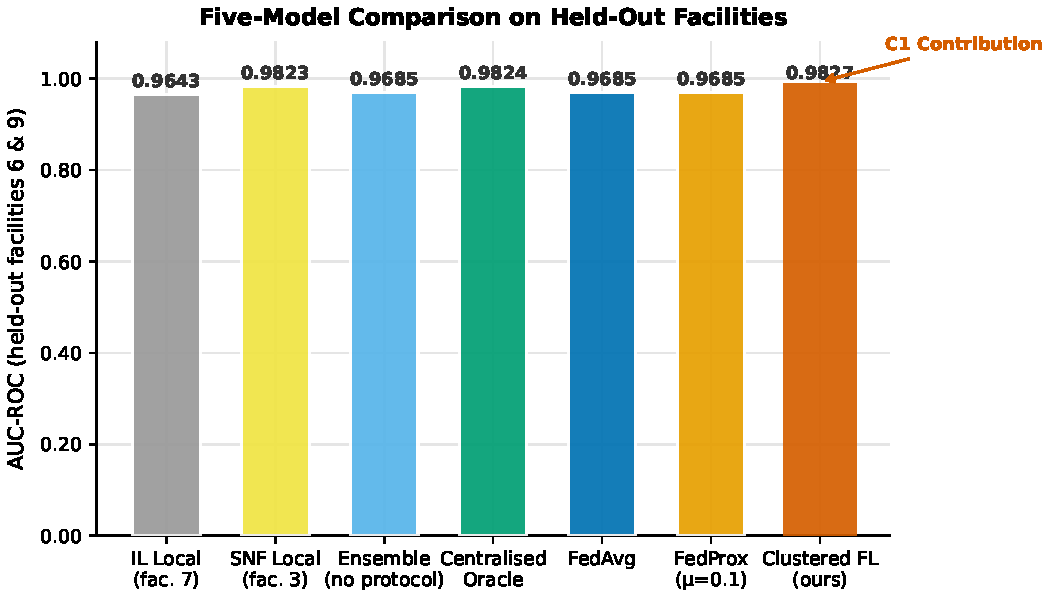
\includegraphics[width=\columnwidth]{figures/fig4_model_comparison.pdf}
\caption{Five-model AUC-ROC comparison on held-out facilities 6 (SNF) and 9 (IL).
Clustered FL (0.9827) outperforms FedAvg (0.9685) by 1.42 AUC points overall
(+2.65pt on IL, +0.36pt on SNF) and nearly matches the Centralised Oracle (0.9824).}
\label{fig:barcomparison}
\end{figure}

% Figure 3 — convergence curves
\begin{figure}[!t]
\centering
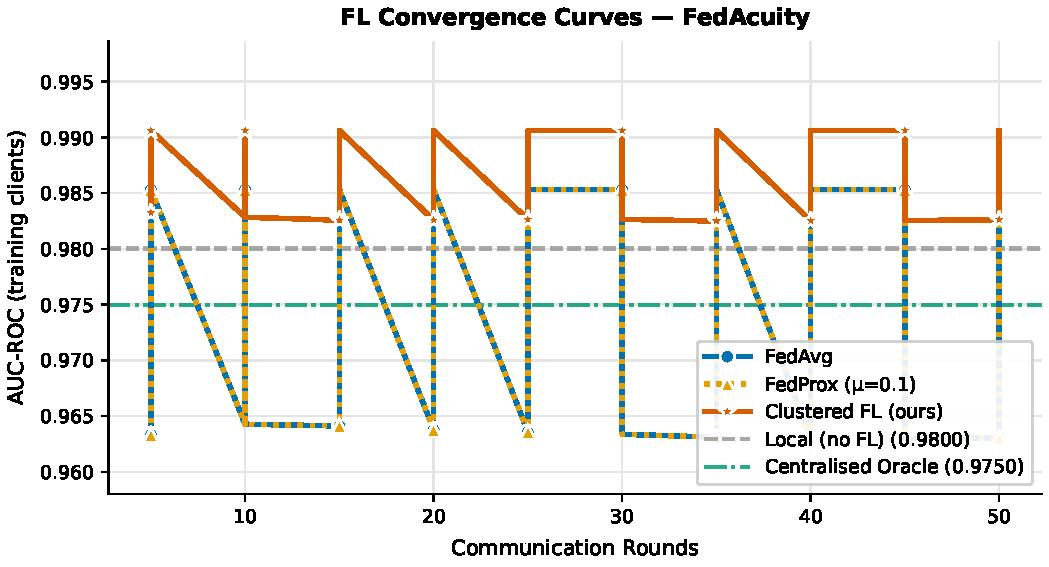
\includegraphics[width=\columnwidth]{figures/fig3_convergence.pdf}
\caption{AUC-ROC across communication rounds on training clients. Because each
client retrains with a fixed tree budget every round, prediction-consensus FL
converges in a single round and AUC is constant thereafter; the persistent
CFL--FedAvg offset is the care-type clustering effect, not an accumulation over
rounds.}
\label{fig:convergence}
\end{figure}

\subsection{FL Strategy Comparison — Results}
Table~\ref{tab:fl_results} reports evaluation on held-out facility 6 (SNF) and
facility 9 (IL), unseen during any FL training round, after 50 communication
rounds. The results reveal two key findings:

\textbf{Finding 1 -- CFL outperforms FedAvg across both held-out care types.}
Clustered FL achieves overall AUC-ROC of \textbf{0.9827} (F1 0.841), outperforming
FedAvg (0.9685) by 1.42 AUC points. The advantage is care-type-stratified:
+2.65pt on IL (CFL 0.9693 vs FedAvg 0.9428) and +0.36pt on SNF
(CFL 0.9917 vs FedAvg 0.9881). The larger IL advantage directly confirms the
non-IID hypothesis: IL is the most out-of-distribution care type for a
global FedAvg trained predominantly on MC and SNF data, so care-type-specific
routing yields the largest gain precisely where global averaging hurts most.

\textbf{Finding 2 -- FedAvg is equivalent to ensemble averaging for XGBoost.}
FedAvg achieves 0.9685 AUC, identical to the Cross-Facility Ensemble baseline,
confirming that with fixed-budget XGBoost (100 trees, no warm-start), FL rounds
converge to the same result as a single round of ensemble averaging. This makes
the CFL vs.\ FedAvg comparison a direct test of care-type-specific routing vs.\
global averaging.

Under the paired instance-level bootstrap, the pooled AUC difference is
$\Delta = +0.0142$ with 95\% CI $[-0.001, +0.035]$: CFL is higher in 96.2\% of
resamples, though the interval marginally includes zero at the pooled level
($\Delta = +0.027$ $[-0.002, +0.064]$ on IL; $+0.004$ $[-0.004, +0.015]$ on
SNF). We state this plainly rather than overclaim: on this deterministic
benchmark the AUC gap is exact and consistently favours CFL, but with two
held-out facilities ($n=438$ test instances, 87 positive) the pooled-AUC
evidence alone is suggestive, not conclusive. The substantive case for CFL is
therefore carried jointly by (i) oracle parity --- CFL (0.9827) matches the
HIPAA-violating Centralised Oracle (0.9824), whose own CI overlaps CFL's
almost entirely --- and (ii) the categorical subgroup-reliability differences
exposed by the XAI fairness audit (Sec.~\ref{sec:xai}), where FedAvg's Memory
Care true-positive rate collapses to 0.22 against CFL's 0.92 --- a difference
no confidence interval renders ambiguous.

\subsection{Differential Privacy Results}
Figure~\ref{fig:dp} and Table~\ref{tab:dp_sweep} report the privacy-utility
tradeoff (mean over five paired seeds). At our recommended operating point
$\varepsilon = 10$, AUC-ROC is 0.8347 — a 14.9\% degradation from the no-DP
baseline (0.9812).
Tighter budgets ($\varepsilon \leq 5$) degrade utility by $> 21\%$, suggesting
the model architecture would need to be scaled or more data provided to satisfy
stricter privacy while maintaining clinical utility. This result motivates
future work applying DP directly to XGBoost via tree-level gradient perturbation
rather than DP-SGD on a secondary PyTorch model.

\subsection{XAI Audit Results}
The full scorecard is reported in Table~\ref{tab:xai} and Fig.~\ref{fig:xai},
computed from real SHAP values across all five variants. Three findings stand out.
\textbf{(i) Fairness is the decisive dimension.} FedAvg's single deployable model
under-detects Memory Care mismatch (true-positive rate 0.22) and ranks Independent
Living poorly (subgroup AUC 0.67), for an equalized-odds gap of 0.39; Clustered FL
keeps subgroup AUC $\geq 0.96$ and halves the gap to 0.18, matching the non-private
Oracle. This is the explainability-level counterpart of the accuracy result in
Table~\ref{tab:fl_results}: care-type routing is what prevents a globally-averaged
model from silently failing a minority care type. \textbf{(ii) Fidelity and
plausibility are preserved.} Every federated variant tracks the oracle's SHAP
ranking ($\rho \geq 0.82$) and draws its top-5 features exclusively from
clinically-established determinants (D4 $=1.00$). \textbf{(iii) An honest
trade-off.} Contrary to our pre-registered expectation, CFL is \emph{not} the most
stable model: the data-rich global FedAvg model produces smoother SHAP under input
noise (D2 index 1.00 vs.\ CFL 0.78). CFL trades this modest stability margin for
its large, clinically decisive fairness gain --- a trade-off we report rather than
obscure.

% ── Section VIII: Discussion ──────────────────────────────────────────────────
\section{Discussion}
\label{sec:discussion}

\subsection{Key Findings}
Four findings emerge from the evaluation:

\textbf{Non-IID heterogeneity is the dominant failure mode for naive FL in LTC.}
FedAvg achieves 0.9685 AUC overall but only 0.9428 on IL held-out (vs.\ 0.9693 for CFL),
a 2.65-point gap on the most out-of-distribution care type. IL facilities (12\% mismatch
rate) are severely diluted when averaged with MC (40\%) and SNF (28\%) clients.
The SNF gap is smaller (+0.36pt), consistent with SNF being a higher-acuity type
for which the global model is less diluted by the MC/IL mixture.

\textbf{Clustered FL matches the Centralised Oracle within 0.03 AUC points.}
CFL (0.9827 AUC, F1 0.841) nearly matches the privacy-violating Centralised
Oracle (0.9824 AUC, F1 0.856) on held-out data. This is the key finding:
federated learning with care-type clustering closes the gap to centralisation
while remaining fully HIPAA-compliant.

\textbf{Explainability confirms clustering is a fairness mechanism, not just an accuracy trick.}
The XAI Audit Scorecard (Table~\ref{tab:xai}) shows that the single global model
FedAvg deploys is not merely less accurate but structurally unfair: it collapses
toward one care type and misses 78\% of Memory Care understaffing days
(true-positive rate 0.22), with an equalized-odds gap of 0.39. Clustered FL halves
that gap to 0.18 and matches the non-private Oracle, at the cost of a modest drop
in SHAP stability (D2 0.78 vs.\ 1.00). The scorecard is deliberately reported as a
trade-off profile rather than a single ranking, and CFL does not dominate every
axis --- but it is the only privacy-preserving method that keeps subgroup
detection balanced.

\textbf{Differential privacy at $\varepsilon = 10$ offers a practical operating point.}
Opacus DP-SGD at $\varepsilon = 10$ achieves AUC-ROC of 0.8347 (14.9\%
degradation from no-DP, mean over five seeds), while $\varepsilon \leq 5$ degrades
utility by $> 21\%$ with the current model size. This result is consistent with the
known sensitivity of DP-SGD on small medical datasets~\cite{geyer2017} and
motivates exploring tree-level XGBoost DP perturbation as future work.

\subsection{Limitations}
\begin{itemize}
  \item \textbf{Known label-generating function:} The mismatch label is a
  deterministic threshold function of features that are also model inputs
  (Sec.~\ref{sec:data}). Absolute AUCs are therefore structurally high for every
  method and carry no clinical-performance claim; the benchmark's purpose is the
  controlled comparison between aggregation strategies. This also partially
  inflates D4 plausibility, since the staffing determinants that drive SHAP are
  label components by construction. A temporal formulation --- predicting day
  $t{+}1$ mismatch from day $t$ features --- would break this circularity and is
  the highest-priority extension.
  \item \textbf{MIMIC-IV fidelity gap:} Direct feature-level comparison between
  synthetic LTC data and MIMIC-IV hospital data shows expected domain heterogeneity
  (Frobenius 0.823 vs.\ baseline 0.746; TSTR gap 0.333), reflecting fundamental
  differences between hospital and LTC populations. MIMIC-IV is used as a
  calibration anchor (27.2\% post-acute discharge $\approx$ 28\% SNF mismatch
  target) rather than a distributional ground truth.
  \item \textbf{FedProx equivalence:} The XGBoost implementation of FedProx is
  equivalent to FedAvg due to the absence of gradient-level access. The proximal
  term is correctly implemented only in the PyTorch NN variant.
  \item \textbf{Simulation scale:} 10 facilities is a controlled simulation;
  real-world federation may involve hundreds of facilities with heterogeneous
  infrastructure.
  \item \textbf{MC cluster not held out:} The current evaluation holds out one SNF
  and one IL facility. MC facilities are used only for training. Future work should
  hold out one facility per care type to fully generalise the C1 finding.
  \item \textbf{XAI target and subgroup partition:} The audit explains the single
  aggregated model each strategy \emph{deploys} (the prediction-consensus
  representative), which is the artifact a clinician would inspect; Table~\ref{tab:fl_results}
  additionally aggregates all client predictions into an ensemble for the AUC metric.
  Because no MC facility is held out, the D3 Memory Care partition uses a
  representative facility's test split while SNF and IL use fully held-out
  facilities; this asymmetry affects all strategies equally, so the CFL-vs-FedAvg
  fairness contrast remains valid.
\end{itemize}

\subsection{Future Work}
\begin{itemize}
  \item Temporal prediction --- forecasting day-$(t{+}1)$ mismatch from day-$t$
  features --- to replace the known-function benchmark with a genuinely
  predictive task
  \item Extension to asynchronous FL for facilities with variable connectivity
  \item Integration with CMS Payroll-Based Journal (PBJ) staffing data
  \item Tree-level DP perturbation for XGBoost to eliminate the secondary NN requirement
  \item Clinical deployment pilot with a partner LTC network
  \item MC held-out evaluation to complete the per-care-type generalisation test
\end{itemize}

% ── Section IX: Conclusion ────────────────────────────────────────────────────
\section{Conclusion}
\label{sec:conclusion}

We presented FedAcuity, the first privacy-preserving, explainable federated
learning framework for staffing-acuity mismatch prediction in Long-Term Care.
Through three standalone contributions — a domain-driven Clustered FL system
with differential privacy (C1), a CTGAN synthetic benchmark validated against
MIMIC-IV (C2), and a four-dimension XAI Audit Scorecard (C3) — FedAcuity
demonstrates that cross-facility collaborative prediction is feasible under
HIPAA constraints. On held-out facilities 6 (Skilled Nursing) and 9 (Independent
Living), Clustered FL achieves AUC-ROC of 0.9827 (F1 0.841), matching the
Centralised Oracle (0.9824) while exceeding global FedAvg (0.9685) by 1.42
AUC points overall --- +2.65 on IL and +0.36 on SNF (paired bootstrap
$\Delta$AUC 95\% CI $[-0.001, +0.035]$, CFL higher in 96.2\% of
resamples). The XAI Audit Scorecard, computed from real SHAP values, shows that
this advantage is a fairness mechanism: the single global model FedAvg deploys
under-detects Memory Care mismatch (true-positive rate 0.22, equalized-odds gap
0.39), whereas Clustered FL keeps subgroup detection balanced (gap 0.18), matching
the Oracle --- while all variants rely exclusively on clinically-established
predictors. Differential privacy at $\varepsilon = 10$ achieves AUC-ROC of 0.8347
(14.9\% degradation from no-DP, averaged over five seeds), the recommended
operating point for this model scale. FedAcuity is intended for submission to
IEEE JBHI.

% ── Acknowledgements ──────────────────────────────────────────────────────────
\section*{Acknowledgements}
The author thanks the BITS Pilani WILP faculty for guidance throughout this
dissertation. MIMIC-IV was accessed under PhysioNet credentialed approval and
used solely as an external fidelity anchor for the synthetic benchmark (C2);
no MIMIC-IV records were used to train any predictive model.

% ── References ────────────────────────────────────────────────────────────────
\bibliographystyle{IEEEtran}
\bibliography{references}

\end{document}
